%!TEX TS-program = xelatex
\documentclass[en]{hust-thesis} % use [vi] for vietnamese

\usepackage{blindtext}
\usepackage{rotating} % For rotating tables
% \usepackage[inline]{enumitem}

\DeclareGraphicsExtensions{.eps, .pdf, .png, .jpeg, .jpg}
\graphicspath{{figures/}{diagrams/}}

\title{Grammatical Error Correction Using Machine Learning Web Application}
\author{Ngô Văn Cảnh}
\authoremail{canh.nv193204@sis.hust.edu.vn}
\major{Electronics and Telecommunications Engineering} % Kỹ thuật điện tử - viễn thông
\field{Electrical and Electronics}
\advisor{Prof. Dương Tấn Nghĩa}
\mentor{Nguyễn Thu Trang}
\department{Department of Electronics Engineering}
\institute{School of Electrical and Electronic Engineering} % Trường Điện - Điện tử
\degree{Thesis}
\university{Hanoi University of Science and Technology}
\universitycity{Hanoi}
\universitystate{Hanoi}
\degreemonth{2}
\degreeyear{2025}

\renewcommand{\glsmcols}{1}
\setglossarystyle{list}

\newacronym{gec}{GEC}{Grammatical Error Correction}
\newacronym{esl}{ESL}{English as a Second Language}
\newacronym{rl}{RL}{Reinforcement Learning}
\newacronym{dl}{DL}{Deep Learning}
\newacronym{ml}{ML}{Machine Learning}
\newacronym{nlp}{NLP}{Natural Language Processing}
\newacronym{bert}{BERT}{Bidirectional Encoder Representations from Transformers}
\newacronym{gpu}{GPU}{Graphics Processing Unit}
\newacronym{s2s}{seq2seq}{Sequence-to-Sequence}

\newglossary[nlg]{notation}{not}{ntn}{Notation}

\newglossaryentry{not:eth}{
  name=\ensuremath{\tilde{E}_{td}},
  description={energy requesting threshold},
  type=notation}

\newglossaryentry{not:bs}{
  name=\ensuremath{p_0},
  description={base station},
  type=notation}

\newglossaryentry{not:snset}{
  name=\ensuremath{\mathcal{P}},
  description={a set of deployed sensors},
  type=notation}

\newglossaryentry{not:num:sn}{
  name=\ensuremath{n},
  description={number of deployed sensors},
  type=notation}

\newglossaryentry{not:sn}{
  name=\ensuremath{p},
  description={a sensor},
  type=notation}


\makeglossaries

\begin{document}

%%%%%%%%%%%%%%%%%%%%%%%%%%%%%%%%
%title
%%%%%%%%%%%%%%%%%%%%%%%%%%%%%%%%
\maketitle
%

\copyrightpage

\authorphone{0383090063}
\authorclass{CTTT Điện tử 01-K64}
\duration{01/09/2024 - 03/02/2025}

\statement{
  This thesis focuses on the development of a web-based application that provides easy access to existing grammatical error correction (GEC) models using advanced natural language processing (NLP) techniques.
  It does not introduce a new GEC method nor improve the performance of existing models.
  Instead, the goal is to make state-of-the-art GEC technology more accessible and user-friendly for the general public by integrating these models into an intuitive and lightweight web interface.
}

\declaration{
  I hereby declare that this thesis is my original work and has not been submitted for any degree or diploma at any other institution.
  Any materials or ideas derived from other sources have been properly cited.
  Furthermore, I declare that there are no conflicts of interest affecting this research.
  % All information cited complies with the intellectual property regulations.
  % The references are clearly listed.
  % I take full responsibility for the content written in this thesis.
}

\requirementpage

\pagenumbering{roman}

\makeatletter
\acknowledgments{
  First and foremost, I would like to express my deepest gratitude to my supervisor, \@advisor, for his invaluable guidance, patience, and unwavering support throughout this journey.
  His insightful feedback and expertise have been instrumental in shaping this thesis.

  I am equally grateful to my mentor, \@mentor, whose dedication and encouragement have been a constant source of motivation.
  Her thoughtful advice and meticulous attention to detail have significantly enhanced the quality of my work.

  And lastly, I extend my heartfelt thanks to my family for their unconditional love, encouragement, and unwavering belief in me.
  Their support has given me the strength and determination to persevere through every challenge.
  This achievement would not have been possible without them.
}
\makeatother


\addcontentsline{toc}{chapter}{Abstract}
\abstractpage{
  This thesis presents a lightweight web application to serve grammatical error correction (from now on refers as GecWeb) systems so that they can be easily used by the general public.
  I design GecWeb to be accessible to as many users as possible, including users who have a slow Internet connection and who use mobile phones as their main devices to connect to the Internet.
  GecWeb provides three state-of-the-art base GEC systems using sequence tagging, as well as two state-of-the-art GEC system combination methods using two approaches (edit-based and text-based).

  % It is suggested to have the abstract in both language (Vietnamese and English).
  \newpage
  \begin{center}
    \vspace*{1pt}
    \Large \textcolor{Crimson}{\textit{Ứng dụng sửa lỗi ngữ pháp sử dụng học máy}} \normalsize\\
    \vspace*{15pt}
    {\bf Tóm tắt đồ án} \rm
  \end{center}

  Luận văn này trình bày một ứng dụng web nhẹ để phục vụ chỉnh sửa lỗi ngữ pháp (sau đây gọi là GecWeb), giúp công chúng dễ dàng tiếp cận và sử dụng.
  GecWeb được thiết kế nhằm đảm bảo khả năng tiếp cận rộng rãi nhất có thể, bao gồm cả những người dùng có kết nối Internet chậm và những người sử dụng điện thoại di động làm thiết bị chính để truy cập Internet.
  GecWeb cung cấp ba hệ thống chỉnh sửa lỗi ngữ pháp (GEC) tiên tiến sử dụng phương pháp gán nhãn chuỗi (sequence tagging), cũng như hai phương pháp kết hợp hệ thống GEC hiện đại dựa trên hai cách tiếp cận khác nhau (dựa trên chỉnh sửa và dựa trên văn bản).
}


\tableofcontents
\addcontentsline{toc}{chapter}{List of Figures}
\listoffigures
\addcontentsline{toc}{chapter}{List of Tables}
\listoftables

\glsaddall
\printglossary[type=\acronymtype,title=List of Acronyms, toctitle=List of Acronyms, nonumberlist]
% \printglossary[type=notation,title=List of Notations, toctitle=List of Notations, nonumberlist]

\newpage
\pagenumbering{arabic}

\chapter{Introduction}

\section{Motivation}
\label{section:motivation}

English is one of the most widely used languages globally, serving as a common medium of communication for over 1.4 billion people worldwide, with almost 75\% of them being non-native speakers~\citep{eberhard2015ethnologue}.
As the number of \acrfull{esl} and \acrfull{efl} learners continues to grow, the demand for effective language learning tools and resources has increased significantly.
However, grammatical and spelling errors remain common challenges for many writers, affecting clarity and professionalism.

\acrfull{gec} is a task that aims to automatically detect and correct errors that are present in a text, including grammatical errors, orthographic errors, misspellings, word choice errors, etc. \citep{ng-etal-2014-conll}

Despite significant recent advancements in GEC technology, many \acrfull{sota} systems remain inaccessible to the general public due to their reliance on command line interfaces and high performance computing resources.
This creates a barrier for non technical users, particularly those in developing countries with limited access to advanced technology and slow internet connections.
The need for a lightweight, user friendly GEC system that can be easily accessed via mobile devices is therefore urgent.

The development of such a system would benefit not only \acrshort{esl} and \acrshort{efl} learners but also native speakers who occasionally make mistakes.
Additionally, improved GEC tools can enhance the quality of other \acrfull{nlp} tasks, such as machine translation and speech recognition, thereby contributing to broader advancements in the field of NLP.

\section{Objectives and scope of the graduation thesis}
\label{section:objective}

Currently, there are several web services, such as those provided by Grammarly and John Snow Labs, offer ready-to-use English text correction.
However, these services are not open-source, limiting their adaptability for deploying different GEC systems.
Therefore, I will only compare and evaluate some available open-source English correction tools, noticeably GECko+ and MiSS.

GECko+ is an English language assisting tool that corrects mistakes of various types in written texts.
It combines a sentence level GEC model, GECToR XLNet, and a sentence ordering model.
When a user inputs a text into the system, it segments the text into sentences and corrects the sentences with GECToR before re-ordering them by the sentence ordering model.
However, GECko+ lacks the options of choosing the GEC base models and using
system combination methods.
It is also unclear how easy it is to extend GECko+ to other GEC systems.

MiSS, on the other hand, is a comprehensive tool for machine translation that includes grammatical error correction as a feature.
The main machine translation features of MiSS include basic machine translation, simultaneous machine translation, and back translation for quality evaluation.
For the GEC part, it uses GECToR XLNet for English GEC and GECToR with BERT-Chinese and BERT-Japanese models for Chinese and Japanese GEC, respectively.
Like GECko+, MiSS also lacks the options of choosing the GEC base models and using system combination methods.

Based on the above analysis, this thesis aims to develop GecWeb (Grammatical Error Correction Web), a web-based application designed to make state-of-the-art GEC systems more accessible to the general public.
GecWeb addresses the limitations of existing GEC tools-such as their reliance on command-line interfaces, lack of mobile support, and limited customization-by offering a lightweight, user-friendly interface.
This application is specifically designed to function efficiently across different screen sizes and varying internet speeds, making it particularly beneficial for users in developing countries.

\section{Tentative solution}
\label{section:tentative}

My proposed solution involves the development of a web application that leverage state-of-the-art GEC models (GECToR-Roberta, GECToR-XlNet and GECToR-Bert) and combination methods, namely ESC (Edit-based System Combination) and MEMT (Multi-Engine Machine Translation).

The front end of GecWeb is built using Flask and Bootstrap, providing a lightweight yet responsive web interface.
Flask was chosen for its simplicity and seamless integration with the back end, while Bootstrap ensures a modern and mobile-friendly user experience.
The back-end is implemented using Flask-RESTful API, which efficiently handles client requests and provides structured API endpoints.
Flask-RESTful was selected due to its minimal overhead, ease of use, and flexibility in designing scalable web services.
The core grammatical error correction functionality is powered by GECToR, a transformer-based machine learning model.
GECToR was chosen because of its state-of-the-art performance in handling complex grammatical errors while maintaining high accuracy and efficiency.

The main contribution of this thesis is the creation of a lightweight, modular GEC system that can be easily extended to include new models and combination methods.
The system will be designed to minimize data transfer overhead, making it suitable for users with slow internet connections.
Furthermore, the system will feature a responsive web interface that adapts to different screen sizes, ensuring a seamless user experience on both desktop and mobile devices.

\section{Thesis organization}
\label{section:organization}

The rest of this graduation thesis is organized as follows.

Chapter 2 focuses on presenting a detailed survey of the current state of GEC systems, including an analysis of user needs and existing products.
This chapter will also outline the functional and non-functional requirements for GecWeb, based on the identified limitations of current systems.

Chapter 3 introduces the methodologies and technologies used in the development of GecWeb.
This chapter will provide an overview of the sequence tagging approaches, as well as the combination methods employed in the system.
The chapter will also discuss the rationale behind the choice of technologies and their relevance to the requirements outlined in Chapter 2.

Chapter 4 discusses in detail the design, implementation, and evaluation of GecWeb.
This chapter will cover the system's architecture, user interface design, and database design.
It will also describe the tools and libraries used in the development process, as well as the testing and deployment of the application.

Chapter 5 presents the solutions and contributions of this thesis, focusing on the innovative aspects of GecWeb and the challenges overcome during its development.
This chapter will highlight the system's modularity, lightweight design, and ability to support multiple GEC models and combination methods.

Finally, Chapter 6 concludes the thesis by summarizing the achievements of GecWeb and discussing potential future work.
This chapter will also provide an analysis of the system's performance compared to existing GEC tools and suggest directions for further improvement.

\chapter{Requirement survey and analysis}

\section{Status survey}
\label{section:2.1}

\section{Functional Overview}
\label{section:2.2}

\subsection{General use case diagram}
\label{subsection:2.2.1}

\subsection{Detailed use case diagram}
\label{subsection:2.2.2}

\subsection{Business process}
\label{subsection:2.2.3}

\section{Functional description}
\label{section:2.3}

\subsection{Description of use case A}
\hfill

\subsection{Description of use case B}
\hfill

\section{Non-functional requirement}
\label{section:2.4}

\chapter{Methodology}
\label{chapter:methodology}

\chapter{Design, implementation, and evaluation}
\label{chapter:design}

This chapter delves deep into the design and implementation of GecWeb, detailing the system's architecture and user interface.

\section{Architecture design}

To make GecWeb more modular, the three-tier architecture, also known as the Model-View-Controller (MVC) architecture, is chosen.
Three-tier architecture is a well-established software application architecture that organizes applications into three logical and physical computing tiers: the presentation tier, or user interface; the application tier, where data is processed; and the data tier, where application data is stored and managed.

The chief benefit of the three-tier architecture is that because each tier runs on its own infrastructure, each tier can be developed simultaneously by a separate development team.
It can be updated or scaled as needed without impacting the other tiers.

\begin{enumerate}
  \item The presentation tier is the user interface and communication layer of the application, where the end user interacts with the application.
        Its main purpose is to display information to and collect information from the user.
        This top-level tier can run on a web browser, as a desktop application, or a graphical user interface (GUI), for example.

  \item The application tier, also known as the logic tier or middle tier, is the heart of the application.
        This tier is responsible for processing user input, making logical decisions, and interacting with the data tier.
        It can also add, delete, or modify data in the data tier.

  \item The data tier is the storage layer of the application, where data is stored, retrieved, and managed.
        This tier can consist of databases, file systems, or other data storage mechanisms.
        The data tier is responsible for managing the application's data and ensuring data integrity and security.
\end{enumerate}

In a three-tier application, all communication goes through the application tier.
The presentation tier and the data tier cannot communicate directly with one another.
Apply this architecture to GecWeb:

\begin{enumerate}
  \item Presentation Layer: The web interface built using Flask and Bootstrap resides in this layer.
  \item It is responsible for rendering the input text box, output text box, and correction highlights.
  \item Application Layer: The Flask RESTful API acts as the controller, handling user requests, managing the selection of GEC models, and coordinating the combination methods.
  \item Data Layer: Although no database is used in GecWeb, the GEC models and combination methods are considered part of the data layer in the context of the three-tier architecture.
        It handles the interaction with the underlying GEC systems and ensures that the corrected text is returned to the application layer.
        The GEC models (GECToR-Bert, GECToR XLNet, GECToR Roberta) and combination methods (ESC, MEMT) reside in this layer.
\end{enumerate}

Although both the GEC models and the web interface can be hosted on the same server, separating them enhances modularity and scalability: the GEC models are hosted on a GPU-powered server, allowing the web interface to run on a CPU-focused server.

\section{Detailed design}

\subsection{System Design and Implementation}

\begin{figure}[htbp]
  \begin{center}
    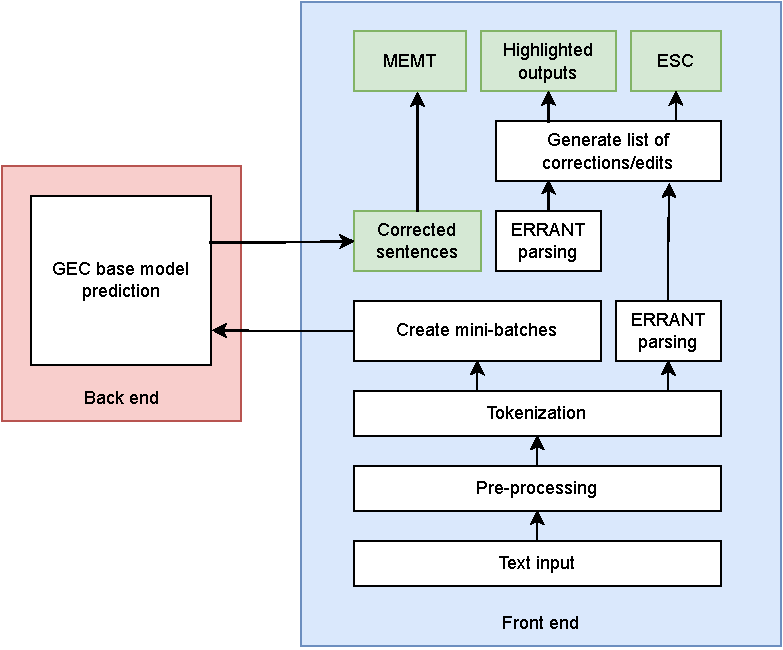
\includegraphics[width=0.7\textwidth]{flowchart}
  \end{center}
  \caption{The process flow of GecWeb}\label{fig:flowchart}
\end{figure}

The process flow of GecWeb is described in Figure~\ref{fig:flowchart}.
All inputs are first split by line and segmented into sentences.
The line index for each sentence is recorded to retain the text structure in the output.
Then, the web interface tokenizes the sentences and combines them into mini-batches to be sent to the base models' API.
If the user chooses to highlight the corrections or combine multiple
base models with ESC, the web interface will also use ERRANT to parse the input sentences.
After receiving the output sentences from each base model, the interface will then parse the base models and outputs using ERRANT if the user chooses to highlight corrections or use ESC.
If not, the outputs are sent to MEMT if the user chooses to combine the models with MEMT.
Otherwise, the output sentences are directly detokenized.
Detokenization also applies to the combination method's output if the user selects more than one base model.

The correction speed of GecWeb is fast.
Running on an NVIDIA Titan X GPU server with 12GB memory, GECToR Roberta can correct text at a speed of 723 words per second, GECToR XLNet at 640 words per second, and GECToR-Bert at 37 words per second.
Using ESC to combine base systems only adds a small amount of overhead.
For example, using ESC to combine GECToR Roberta and GECToR-Bert can correct text at a speed of 32 words per second, marginally slower than using GECToR-Bert alone.

\subsection{User interface design}

The user interface of GecWeb is designed to be responsive and accessible across various screen resolutions, ensuring a seamless experience for users on different devices.
The layout adapts to screens as small as 320x480 pixels, commonly found on mobile phones, up to 1920x1080 pixels, which is standard for desktop monitors.
To maintain accessibility, the color scheme adheres to a contrast ratio above 4.5:1, ensuring readability for users with visual impairments.

Consistency and standardization are key aspects of the interface design.
Buttons maintain a uniform appearance with rounded corners and consistent padding, providing a visually appealing and user-friendly experience.
The "Run" button, which triggers the grammatical error correction process, is prominently displayed in a contrasting color, making it easily identifiable.
Feedback messages, including error notifications and success confirmations, appear at the top of the screen, ensuring they are immediately visible to users.

The color scheme follows a clean and intuitive design, primarily using shades of blue, green, and white.
Corrections made to the text are highlighted in green to enhance visibility, allowing users to easily identify the suggested changes.
This structured approach to design improves usability, ensuring that the interface remains simple, effective, and accessible to a wide range of users.

\section{Application Building}

\subsection{Libraries and Tools}

Table~\ref{tab:tools} provides a comprehensive list of all the tools and libraries that I have used in the development of GecWeb, along with their versions and URLs for more information.

\begin{sidewaystable}[htbp]
  \caption{Tools and libraries}\label{tab:tools}
  \raggedleft
  \begin{tabular}{|l|l|l|l|}
    \hline
    Name             & Purpose                                & Version     & URL                                              \\ \hline
    WSL              & Linux environment                      & 2.3.26.0    & <https://learn.microsoft.com/en-us/windows/wsl/> \\ \hline
    Neovim           & Text editor/IDE                        & 0.10.3      & <https://github.com/neovim/neovim>               \\ \hline
    Conda            & Package, environment management system & 24.7.1      & <https://anaconda.org/anaconda/conda>            \\ \hline
    Python           & Programming language                   & 3.10.16     & <https://github.com/python/cpython>              \\ \hline
    Pyright          & Static Type Checker for Python         & 1.1.391     & <https://github.com/microsoft/pyright>           \\ \hline
    Ruff             & Linter and formatter for Python        & 0.8.4       & <https://github.com/astral-sh/ruff>              \\ \hline
    Pytest           & Unit test frameworks                   & 8.3.4       & <https://github.com/pytest-dev/pytest>           \\ \hline
    Curl             & Test API endpoints                     & 8.11.1      & <https://github.com/curl/curl>                   \\ \hline
    Windows Terminal & Terminal                               & 1.21.3231.0 & <https://github.com/microsoft/terminal>          \\ \hline
    Tmux             & Terminal Multiplexer                   & 3.5a        & <https://github.com/tmux/tmux/wiki>              \\ \hline
    Git              & Version control system                 & 2.45.2      & <https://git-scm.com/>                           \\ \hline
    Docker           & Containerization and Virtualization    & 24.7.0      & <https://www.docker.com/>                        \\ \hline
    Flask            & Web Framework                          & 3.1.0       & <https://flask.palletsprojects.com/>             \\ \hline
    Bootstrap        & Front-End                              & 5.2.3       & <https://getbootstrap.com/>                      \\ \hline
  \end{tabular}
\end{sidewaystable}

\subsection{First prototype}

As mentioned in Chapter 2, Gradio was used to build the first protype of GecWeb.
The user interface of this prototype is shown in Figure~\ref{fig:prototype}.

\begin{figure}[htbp]
  \begin{center}
    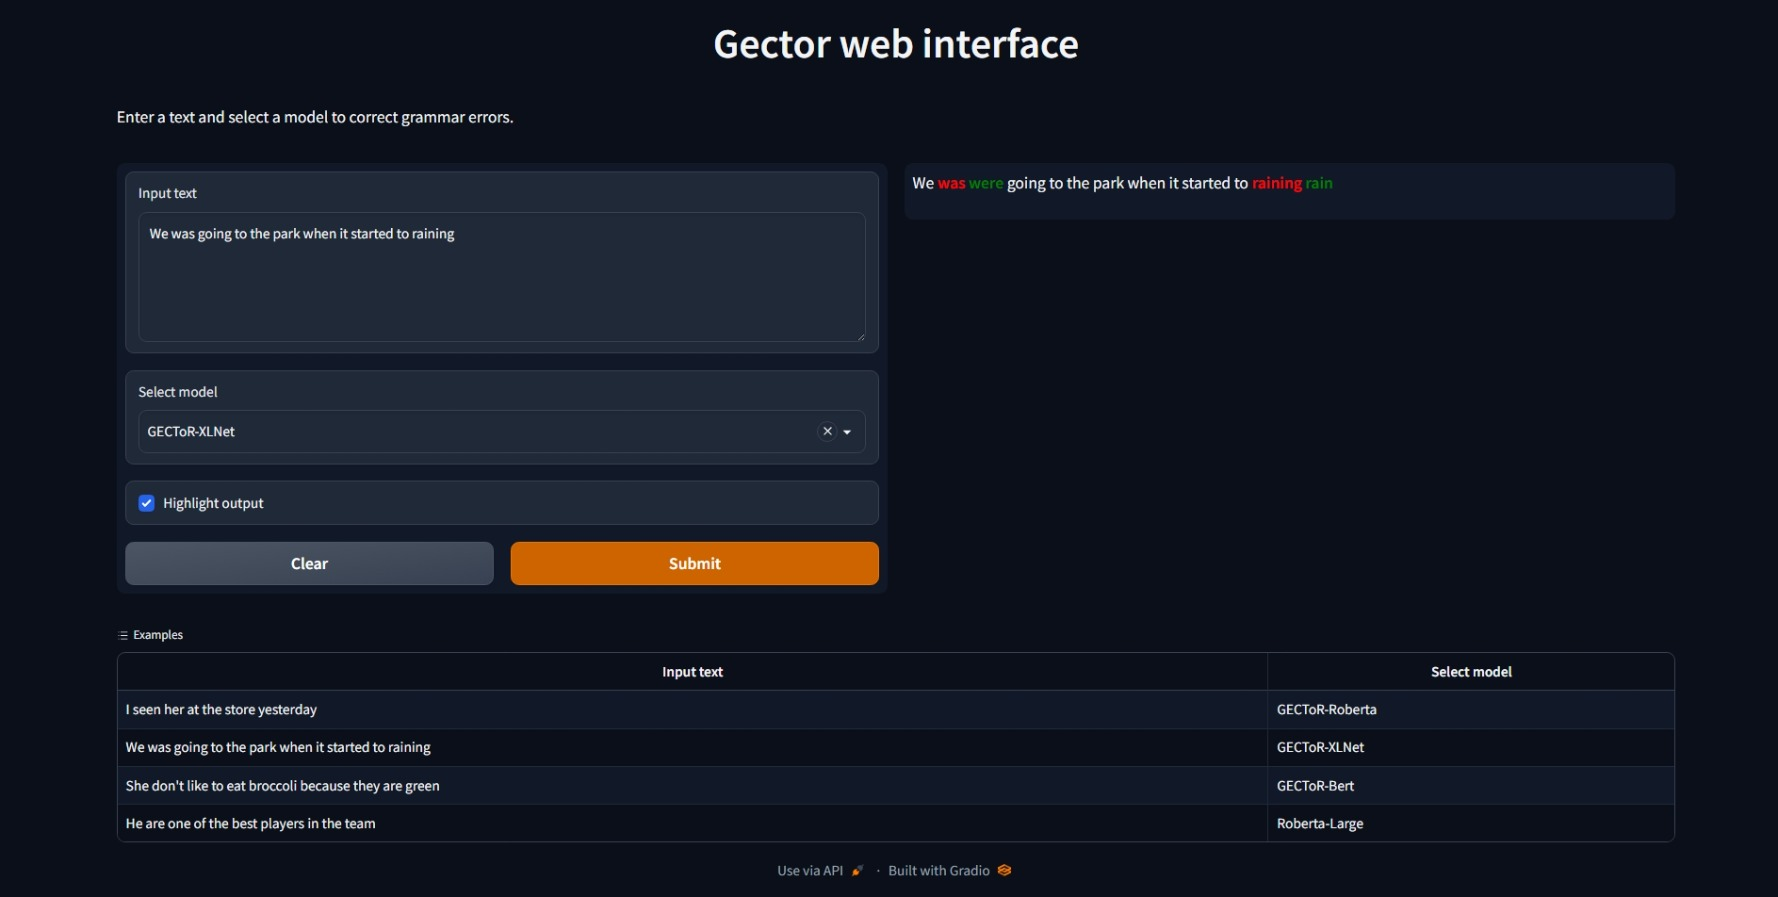
\includegraphics[width=\textwidth]{prototype}
  \end{center}
  \caption{First prototype of GecWeb}\label{fig:prototype}
\end{figure}

In this prototype, the system combination method is not yet implemented.
Additionally, both the models and the interface is run in the same machine.
Although it lack some functionality that I specified in Chapter 2, it provides a quick demo of GecWeb.
You can still access this version on \href{https://huggingface.co/spaces/canh25xp/gector_demo}{My Hugging Face page}
To reduce resources used, the app auto put it self to sleep after 24 hours of inactivity.
So you might have to wait for 10-20s for the app to boot up.

\subsection{Illustration of GecWeb}

The interface of GecWeb consists of five components, which are (i) base model selection, (ii) combination method selection, (iii) output mode, (iv) input text box, and (v) output text box.
The user interface of GecWeb is shown in Figure~\ref{fig:home}.
You might notice that GecWeb bears some resemblance to Google Translate, with the app name at the top, an input box on the left, and an output box on the right.
This similarity is because GecWeb's design is heavily inspired by Google Translate, given that both applications perform text-to-text transformations.

\begin{figure}[htbp]
  \begin{center}
    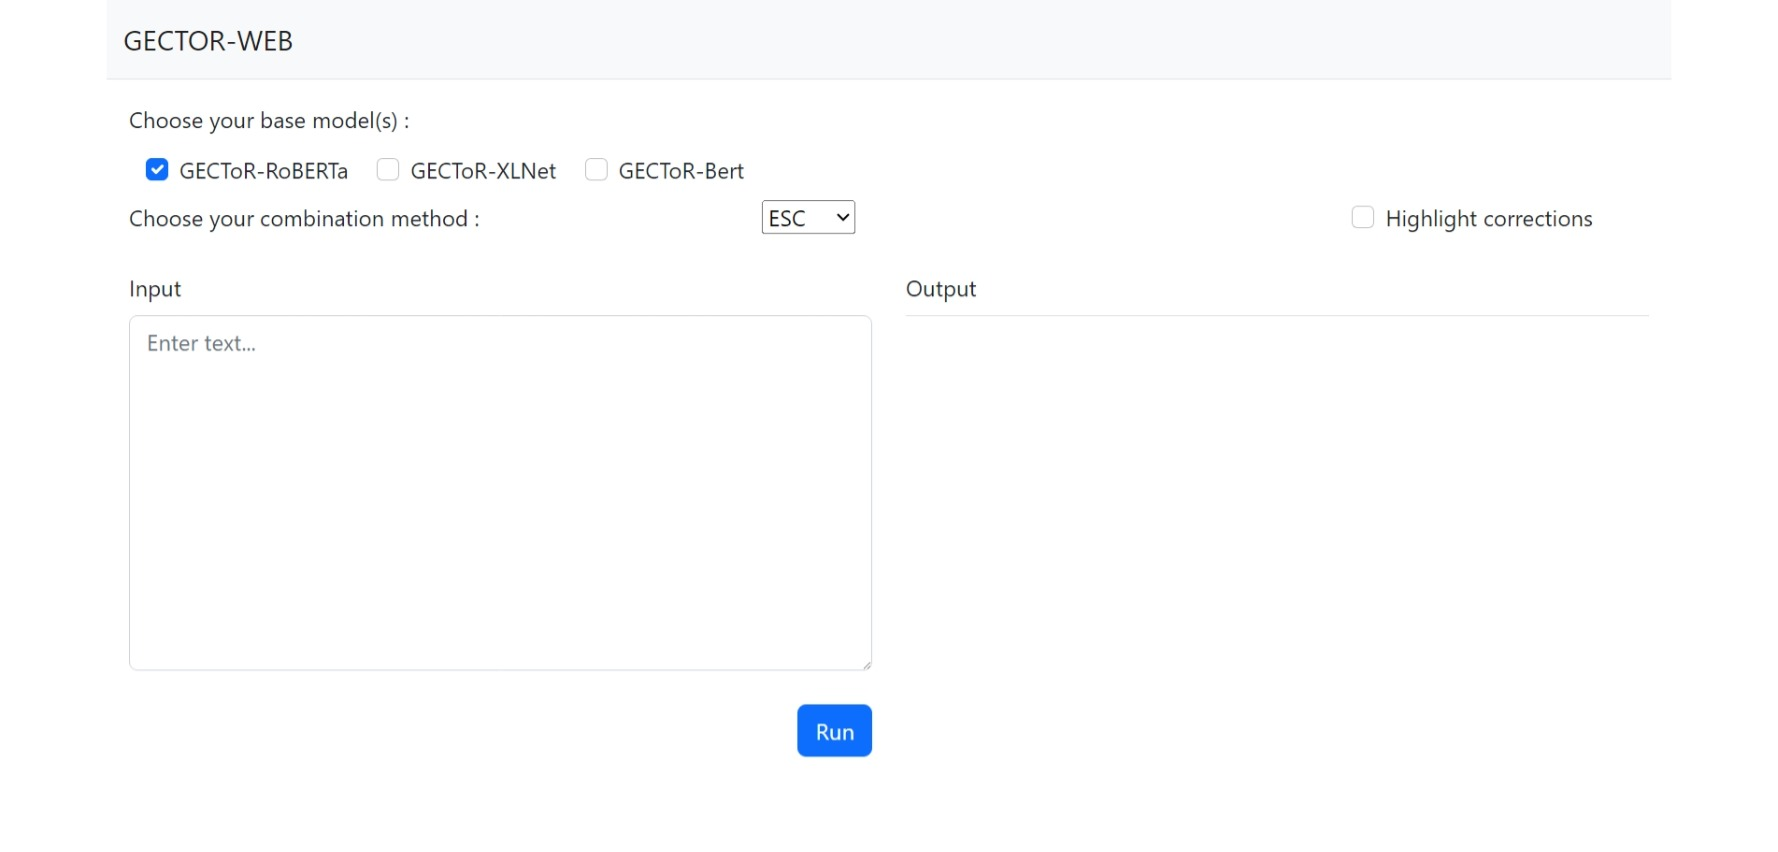
\includegraphics[width=\textwidth]{home}
  \end{center}
  \caption{The User Interface of GecWeb.}\label{fig:home}
\end{figure}

\subsubsection{Base Model Selection}

The user first needs to choose the base model(s).
If the user chooses more than one base model, GecWeb will run a system combination method based on the combination method selected, as described in Chapter 3.

\subsubsection{Combination Method Selection}

Next, the user needs to choose the combination method.
If the user only chooses one base system, the selected combination method is ignored.
As mentioned earlier in Chapter 3, GecWeb includes two state-of-the-art system combination methods, ESC and MEMT.

\subsubsection{Output Mode}

Users can choose to highlight the corrections by selecting the "Highlight corrections" box.
If the user chooses to highlight the corrections, text spans in the output text that are different from the input text are highlighted in green and a simple explanation of each correction can be displayed by clicking a highlighted text span.
The appearance of highlighted corrections can be seen in Figure~\ref{fig:highlight}.
Displaying corrections with simple explanations can help language learners to understand their mistakes better.
I extracted the corrections with their edit types using ERRANT.

\begin{figure}[htbp]
  \begin{center}
    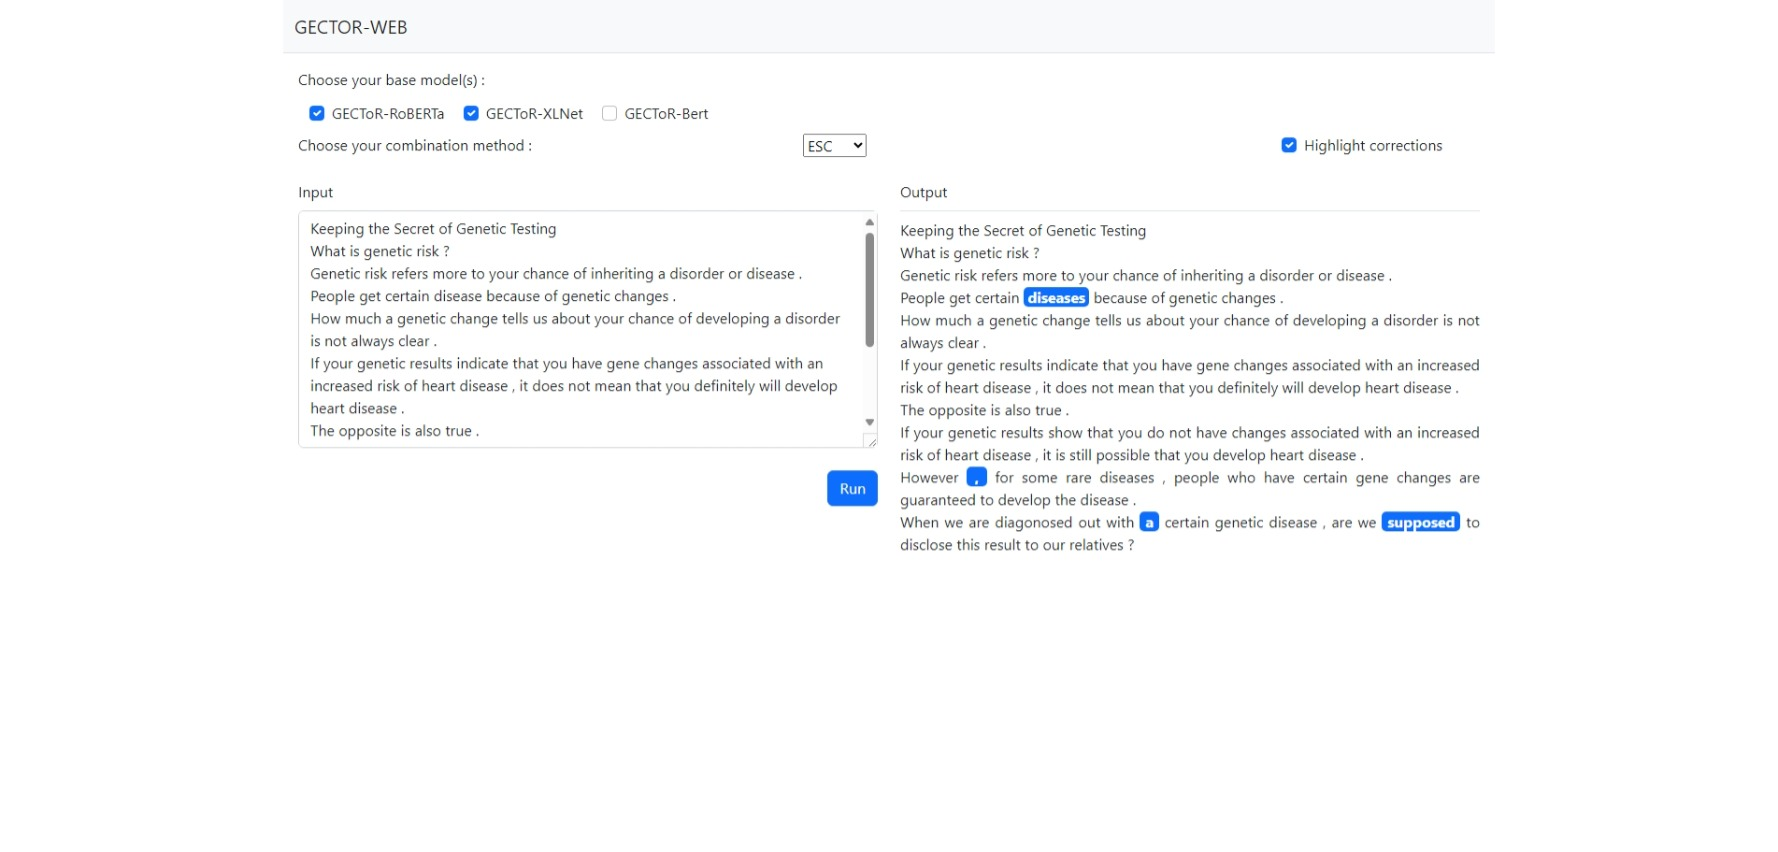
\includegraphics[width=\textwidth]{highlight}
  \end{center}
  \caption{The interface with highlighted corrections, showing green highlights for corrected text and explanations for each correction.}\label{fig:highlight} \end{figure}

\subsubsection{Input Text Box}

The user needs to put the text they want to correct in the input text box and clicks the run button.
The corrected text will then be displayed in the output text box.
Most recent GEC base systems expect the input to be a single sentence tokenized with SpaCy version 1.9, following the requirement from the BEA-2019 shared task.
As such, an input text needs to be segmented into sentences and then tokenized with SpaCy before each sentence is given as the input to the GEC model.
To retain the text structure, it is first split by line before segmented into sentences.
This way, I can keep the information on which line a sentence should be printed.
To segment a text into sentences, I follow the practice used in the NUCLE corpus by using the nltk Punkt
tokenizer.

\subsubsection{Output Text Box}

After a text is entered into the input text box and the "Run" button is clicked, the corrected text will appear in the output text box.
As the base GEC systems are expected to work on tokenized input and output, the output text needs to be detokenized to look more natural.
Since SpaCy does not have a detokenizer and the document context of the original input may no longer be relevant after a sentence is corrected, I use Moses todetokenize a sentence.
I found that Moses can detokenize a sentence that is tokenized by SpaCy reasonably well, only missing some cases like the detokenization of "is n't" and "are n;t" and removing spaces around hyphens.
For these missed cases, I create simple rules to apply string replacement after Moses detokenization.
Detokenization is not applied if the user chooses to highlight the corrections because the highlights need some room to make them clearly visible.

\section{Testing}

The back-end contains several test methods, with both automated and manual testing conducted to ensure the correctness and reliability of the system.
The unit tests are implemented using pytest, a popular testing framework in Python.

% These tests focus on verifying the behavior of individual components of the back-end, namely:
%
% \begin{enumerate}[label=(\roman*)]
%   \item test\_bert\_embedder.py
%   \item test\_gec\_model.py
%   \item test\_gec\_predictor.py
%   \item test\_roberta\_embedder.py
%   \item test\_seq2labels.py
%   \item test\_token\_indexer.py
%   \item test\_tokenization.py
% \end{enumerate}

The Test Token Embedder for BERT Model ensures that the token embedding process for the BERT model functions correctly, validating that the input text is properly tokenized and converted into embeddings that the model can process.
Similarly, the Test Token Embedder for RoBERTa Model performs the same validation for the RoBERTa model, ensuring compatibility with different transformer-based architectures.
The Test Class for GecModel verifies the core functionality of the grammatical error correction model, including its ability to process input text and generate corrections.
Additionally, the Test Class for Seq2Labels Model ensures that the sequence-to-labels model, which is used for sequence tagging tasks, operates as expected.

In addition to unit tests, regression testing is performed to ensure that changes to the codebase do not introduce unintended side effects.
The regression tests use the GECToR-Roberta model to generate predictions for all test files and verify that there are no changes in the output.
This is particularly important for maintaining the consistency of the system, especially when updates or modifications are made to the models or the back-end logic.
The regression tests help ensure that the system's performance remains stable over time and that any new changes do not degrade the quality of the corrections.

To further streamline the testing process, both the unit tests and regression tests are automated using GitHub Actions in multiple Python environments (3.8, 3.9, and 3.10) to ensure compatibility across different versions.
The tests are triggered automatically whenever code is pushed to the main branch, ensuring continuous integration and preventing faulty code from being merged.

Finally, manual API testing is conducted using curl to interact with the back-end API directly, further confirming the proper functioning of the web service.

\section{Deployment}

The deployment of GecWeb is designed to ensure efficient access to grammatical error correction while leveraging the computing power of GPU-focused servers.
The system consists of two main components: the Gec API, which handles the processing of text corrections, and the Gec Web interface, which provides users with an interactive front end to access the correction features.

The Gec API is hosted on Hugging Face Inference Endpoints, which provide dedicated GPU resources to efficiently run deep learning models.
Since grammatical error correction models, such as GECToR, require significant computational power for inference, deploying the API on GPU-accelerated infrastructure ensures fast response times and scalability.
By hosting the API on Hugging Face Inference Endpoints, the system benefits from automatic scaling, secure deployment, and optimized performance without requiring extensive server management.

The Gec Web interface is hosted separately on Hugging Face Spaces, a platform designed for hosting interactive web applications.
Spaces allow developers to easily deploy front-end applications built with frameworks like Flask and Bootstrap, providing a simple way to share machine-learning models with the public.
Hosting GecWeb on Spaces ensures that users can access the interface without requiring local installations, making the system widely accessible.
The front-end communicates with the Gec API by sending text data for processing and receiving corrected outputs, ensuring a seamless and responsive user experience.

By separating the back-end processing from the front-end interface, the deployment strategy optimizes performance and usability.
The API benefits from high-performance GPUs, while the web interface remains lightweight and accessible through any modern browser.
This cloud-based approach allows for easy updates, maintenance, and potential future expansions, making GecWeb an efficient and user-friendly platform for grammatical error correction.


\chapter{Solution and contribution}
\label{chapter:contribution}

\chapter{Conclusion and future work}
\label{chapter:conclusion}

In this thesis, I have presented GecWeb, a web-based application for GEC that can be easily used by the general public.
GecWeb designed to be accessible to as many users as possible, including users who have a slow Internet connection and who use mobile phones as their main devices to connect to the Internet.
In GecWeb, I provide three base GEC systems using sequence tagging, as well as two GEC system combination methods from two types of approaches, edit-based and text-based combination.
GecWeb is separated into two parts to make the application modular and easily extensible to other base GEC systems.

GecWeb is currently limited to English GEC systems, but it can be extended to other languages by incorporating base GEC models for other languages and modifying the pre-processing and post processing steps.


\clearpage
\bibliography{refs}
\addcontentsline{toc}{chapter}{References}
\bibliographystyle{plainnat}

% \begin{appendices}
%   \chapter{This is title of appendix A}
\blindmathpaper
%   \chapter{This is title of appendix B}
\blindmathpaper
% \end{appendices}

\end{document}
